% mnras_template.tex 
%
% LaTeX template for creating an MNRAS paper
%
% v3.0 released 14 May 2015
% (version numbers match those of mnras.cls)
%
% Copyright (C) Royal Astronomical Society 2015
% Authors:
% Keith T. Smith (Royal Astronomical Society)

% Change log
%
% v3.0 May 2015
%    Renamed to match the new package name
%    Version number matches mnras.cls
%    A few minor tweaks to wording
% v1.0 September 2013
%    Beta testing only - never publicly released
%    First version: a simple (ish) template for creating an MNRAS paper

%%%%%%%%%%%%%%%%%%%%%%%%%%%%%%%%%%%%%%%%%%%%%%%%%%
% Basic setup. Most papers should leave these options alone.
\documentclass[fleqn,usenatbib,letters]{mnras}

% MNRAS is set in Times font. If you don't have this installed (most LaTeX
% installations will be fine) or prefer the old Computer Modern fonts, comment
% out the following line
\usepackage{newtxtext,newtxmath}
% Depending on your LaTeX fonts installation, you might get better results with one of these:
%\usepackage{mathptmx}
%\usepackage{txfonts}

% Use vector fonts, so it zooms properly in on-screen viewing software
% Don't change these lines unless you know what you are doing
\usepackage[T1]{fontenc}
\usepackage{ae,aecompl}


%%%%% AUTHORS - PLACE YOUR OWN PACKAGES HERE %%%%%

% Only include extra packages if you really need them. Common packages are:
\usepackage{graphicx}	% Including figure files
\usepackage{amsmath}	% Advanced maths commands
\usepackage{amssymb}	% Extra maths symbols

%%%%%%%%%%%%%%%%%%%%%%%%%%%%%%%%%%%%%%%%%%%%%%%%%%

%%%%% AUTHORS - PLACE YOUR OWN COMMANDS HERE %%%%%

% Please keep new commands to a minimum, and use \newcommand not \def to avoid
% overwriting existing commands. Example:
%\newcommand{\pcm}{\,cm$^{-2}$}	% per cm-squared

%%%%%%%%%%%%%%%%%%%%%%%%%%%%%%%%%%%%%%%%%%%%%%%%%%

%%%%%%%%%%%%%%%%%%% TITLE PAGE %%%%%%%%%%%%%%%%%%%

% Title of the paper, and the short title which is used in the headers.
% Keep the title short and informative.
\title[An orbit for FSR1758]{An orbit for FSR1758}

% The list of authors, and the short list which is used in the headers.
% If you need two or more lines of authors, add an extra line using \newauthor
\author[Simpson et al.]{
Jeffrey D. Simpson$^{1}$\thanks{E-mail: jeffrey.simpson@unsw.edu.au}
\\
% List of institutions
$^{1}$School of Physics, UNSW, Sydney, NSW 2052, Australia
}

% These dates will be filled out by the publisher
\date{Accepted XXX. Received YYY; in original form ZZZ}

% Enter the current year, for the copyright statements etc.
\pubyear{2019}

% Don't change these lines
\begin{document}
\label{firstpage}
\pagerange{\pageref{firstpage}--\pageref{lastpage}}
\maketitle

% Abstract of the paper
\begin{abstract}
We present an orbital calculation for the newly characterized stellar object FSR1758. This shows an object for a large motion out of the bulge and the plane of the Galaxy, with a radial distance varying from 4--16~kpc.
\end{abstract}

% Select between one and six entries from the list of approved keywords.
% Don't make up new ones.
\begin{keywords}
keyword1 -- keyword2 -- keyword3
\end{keywords}

%%%%%%%%%%%%%%%%%%%%%%%%%%%%%%%%%%%%%%%%%%%%%%%%%%

%%%%%%%%%%%%%%%%% BODY OF PAPER %%%%%%%%%%%%%%%%%%

\section{Introduction} \label{sec:intro}
Recently \citet{Barba2018} presented a physical characterization of the large, massive stellar object FSR1758. Using a combination of astrometry and photometry from Gaia, DECaPS, and VVVX, they found the stellar cluster to be curiously large and could potentially be the stripped core of a dwarf galaxy. As noted by the authors, one of the key pieces of information missing were spectroscopic observations of the cluster. These are crucial for deriving a full orbit and for confirming the photometric metallicity.

In this letter we present an analysis of the orbit of FSR1758 based upon four member stars that have radial velocities (RVs) from the Gaia Radial Velocity Spectrometer (RVS).

\section{Data}

%% The "ht!" tells LaTeX to put the figure "here" first, at the "top" next
%% and to override the normal way of calculating a float position
\begin{figure*}
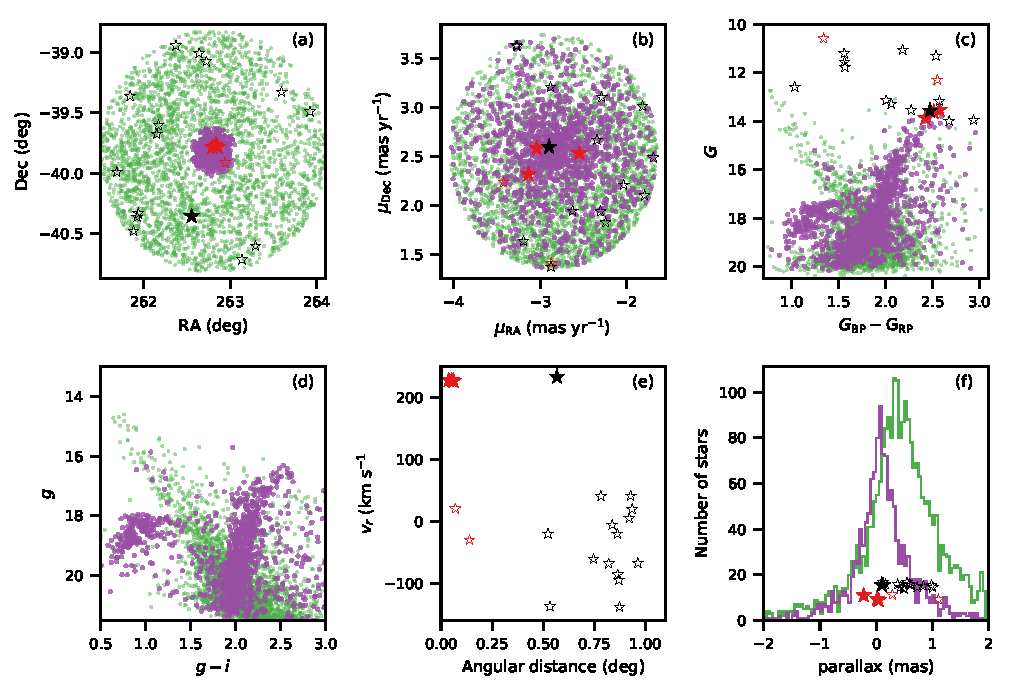
\includegraphics[width=\textwith]{figures/cmd.pdf}
\caption{Colour-magnitude diagram of FSR1758. Blue points indicate those stars that pass the positional and proper motion criteria. The black dots are all stars within 1.5 degrees that pass just the proper motion criterium. Shown with red stars are the four members with radial velocities. \label{fig:cmd}}
\end{figure*}

An initial search was conducted for all Gaia DR2 targets within 1.0 degrees of $\mathrm{RA}=262.806^\circ, \mathrm{Dec}=-39.822^\circ$, which returned a catalogue of over 1.5 million stars.

The cluster has a distinct proper motion \citep{Cantat-Gaudin2018, Barba2018}, and an initial sample of likely cluster members can be identified using a positional and proper motion cuts. We select our `cluster' sample as those stars within 0.20 degrees of the position, and with proper motions within 1.2 mas/yr of proper motion found by \citet{Barba2018}: $(\mu_\mathrm{RA},\mu_\mathrm{Dec})=(-2.85,2.55)$~mas/yr.

Within this sample of 1345 stars, there were five with radial velocities, with three having $226<v_r<228$~km/s. The other two stars had RV like that which would be expected along the line-of-sight --- i.e., $-100<v_r<75$~km/s. And these three stars with high RV were all found at the tip of the RGB of FSR1758. \citet{Barba2018} estimated the tidal radius to be $0.78\pm0.22$~deg, so we extended the search for possible members further out. Within the surrounding 1~deg, there is one further star with a large RV, which again is consistent with the tip of the GB. 

This found four stars with radial velocities: , and one at about 20~km/s. These stars are plotted on the colour-magnitude diagram in Figure \ref{}. The three stars with the large RV are consistent with being bright GB members of FSR1758, while the star with the discrepant RV is found to be about a magnitude brighter than the tip of the GB. We conclude that FSR1758 has an RV of 227~km/s.

Unfortunately the RUWE of one of these cluster members is 1.7. \citep{Lindegren2018}.


\section{Orbit and possible tidal stellar stream}

\begin{figure*}
	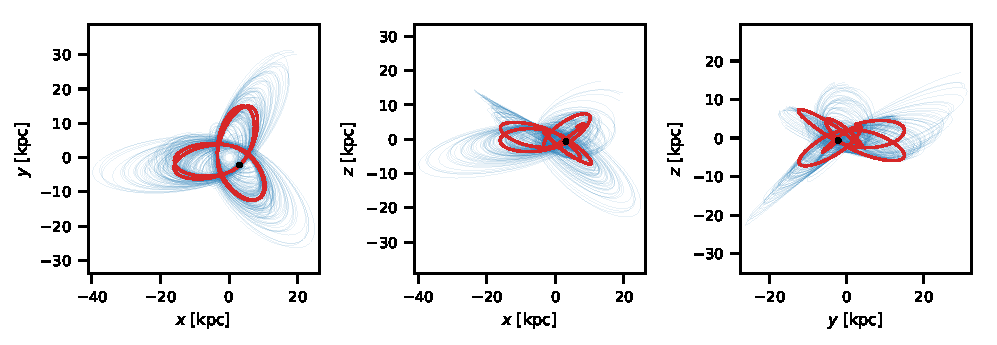
\includegraphics[width=\textwith]{figures/orbit.pdf}
    \caption{\label{fig:orbit}}
\end{figure*}

With a radial velocity, it is now possible to calculate a possible orbit for FSR1758. We use the \textsc{gala} (version 0.3) to compute the orbit \citep{M.Price-Whelan2017,Price-Whelan2018b}, with the default potential \texttt{MilkyWayPotential}. This is a simple mass-model for the Milky Way consisting of a spherical nucleus and bulge, a Miyamoto-Nagai disk, and a spherical NFW dark matter halo. The parameters of this model are set to match the circular velocity profile and disk properties of \citet{Bovy:2015gg}. We place the Sun at a Galactocentric distance of 8.2~kpc, and height above the plane of 25~pc \citep{BlandHawthorn:2016iq, Bland-hawthorn2018}. The Sun's velocity were $(U_\odot,V_\odot,W_\odot)=(11,248,7.25)$~km/s \citep{Schonrich2012}. The cluster position and velocity were $(\alpha,\delta,D_\odot,\mu_\mathrm{RA},\mu_\mathrm{Dec},v_r)=(262.806^\circ,-39.822^\circ,11.5\pm1.0~\mathrm{kpc},-2.85\pm0.1~\mathrm{mas/yr},2.55\pm0.1~\mathrm{mas/yr},227\pm1~\mathrm{km/s})$. 

In Figure \ref{fig:orbit} is the plot of the previous 5 Gyr of the orbit of FSR1758. The cluster is found to have a radial orbit, with a pericenter of $3.84_{-0.90}^{+0.89}$~kpc, an apocenter of $16.60_{-5.46}^{+7.74}$~kpc, and eccentricity of $0.62_{-0.04}^{+0.05}$. In Figure \ref{fig:other_clusters} these values are placed in context of the rest of the Galactic globular cluster population.

% % Example figure
% \begin{figure}
% 	% To include a figure from a file named example.*
% 	% Allowable file formats are eps or ps if compiling using latex
% 	% or pdf, png, jpg if compiling using pdflatex
% 	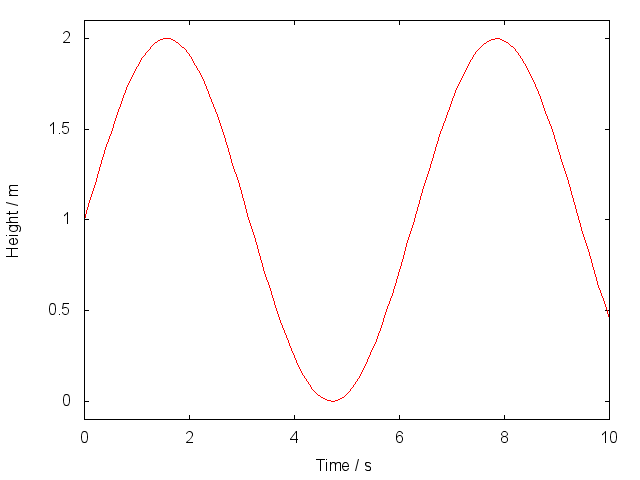
\includegraphics[width=\columnwidth]{example}
%     \caption{This is an example figure. Captions appear below each figure.
% 	Give enough detail for the reader to understand what they're looking at,
% 	but leave detailed discussion to the main body of the text.}
%     \label{fig:example_figure}
% \end{figure}

% % Example table
% \begin{table}
% 	\centering
% 	\caption{This is an example table. Captions appear above each table.
% 	Remember to define the quantities, symbols and units used.}
% 	\label{tab:example_table}
% 	\begin{tabular}{lccr} % four columns, alignment for each
% 		\hline
% 		A & B & C & D\\
% 		\hline
% 		1 & 2 & 3 & 4\\
% 		2 & 4 & 6 & 8\\
% 		3 & 5 & 7 & 9\\
% 		\hline
% 	\end{tabular}
% \end{table}


\section{Discussion}

Unfortunately there do not appear to have been any more serendipitous spectroscopic observations of members of this cluster. In the case of the large all-sky surveys RAVE \citep{Kunder:2017gp} and GALAH \citep{DeSilva:2015gr,Buder2018}, the FSR1758 is too far into the Galactic plane for their observing footprints. Searches of the AAT, ESO, or Gemini archives fail to find any likely observations of cluster members made during bulge star surveys.

We reiterate the words of \citet{Barba2018} that ``acid test for this cluster will be to obtain spectra for a number of members''. This will enable a much better characterization of its line-of-sight velocity dispersion and metallicity, and other abundance distributions. With only four stars, it is not possible to make any comments about the radial velocity dispersion, and therefore the mass-to-light ratio of FSR1758.

\section*{Acknowledgements}

JDS acknowledges the support of the Australian Research Council through Discovery Project grant DP180101791.

%%%%%%%%%%%%%%%%%%%%%%%%%%%%%%%%%%%%%%%%%%%%%%%%%%

%%%%%%%%%%%%%%%%%%%% REFERENCES %%%%%%%%%%%%%%%%%%

% The best way to enter references is to use BibTeX:

\bibliographystyle{mnras}
\bibliography{/Users/jeffrey/Documents/library.bib}

%%%%%%%%%%%%%%%%%%%%%%%%%%%%%%%%%%%%%%%%%%%%%%%%%%

%%%%%%%%%%%%%%%%% APPENDICES %%%%%%%%%%%%%%%%%%%%%

\appendix

\section{Some extra material}

If you want to present additional material which would interrupt the flow of the main paper,
it can be placed in an Appendix which appears after the list of references.

%%%%%%%%%%%%%%%%%%%%%%%%%%%%%%%%%%%%%%%%%%%%%%%%%%


% Don't change these lines
\bsp	% typesetting comment
\label{lastpage}
\end{document}

% End of mnras_template.tex